\chapter{Work and Energy}


Energy is what makes things happen: it moves cars, heats soup, and lights your phone screen. Work is how energy gets from one thing to another. Both ideas start with force, which, as you know, is measured in newtons.

\section{Work}
When you lean on a wall, you are exerting a force on the wall, but you
are not doing any work. On the other hand, if you push a car for a mile,
you are clearly doing work, as in Figure~\ref{fig:workvsforce}. Work, to an engineer, is the force you
apply to something, as well as the distance that something moves, in the direction
of the applied force. We measure work in \textit{joules}. A joule is one
newton of force applied over one meter.\index{Joule}
\begin{figure}[H]
    \centering
    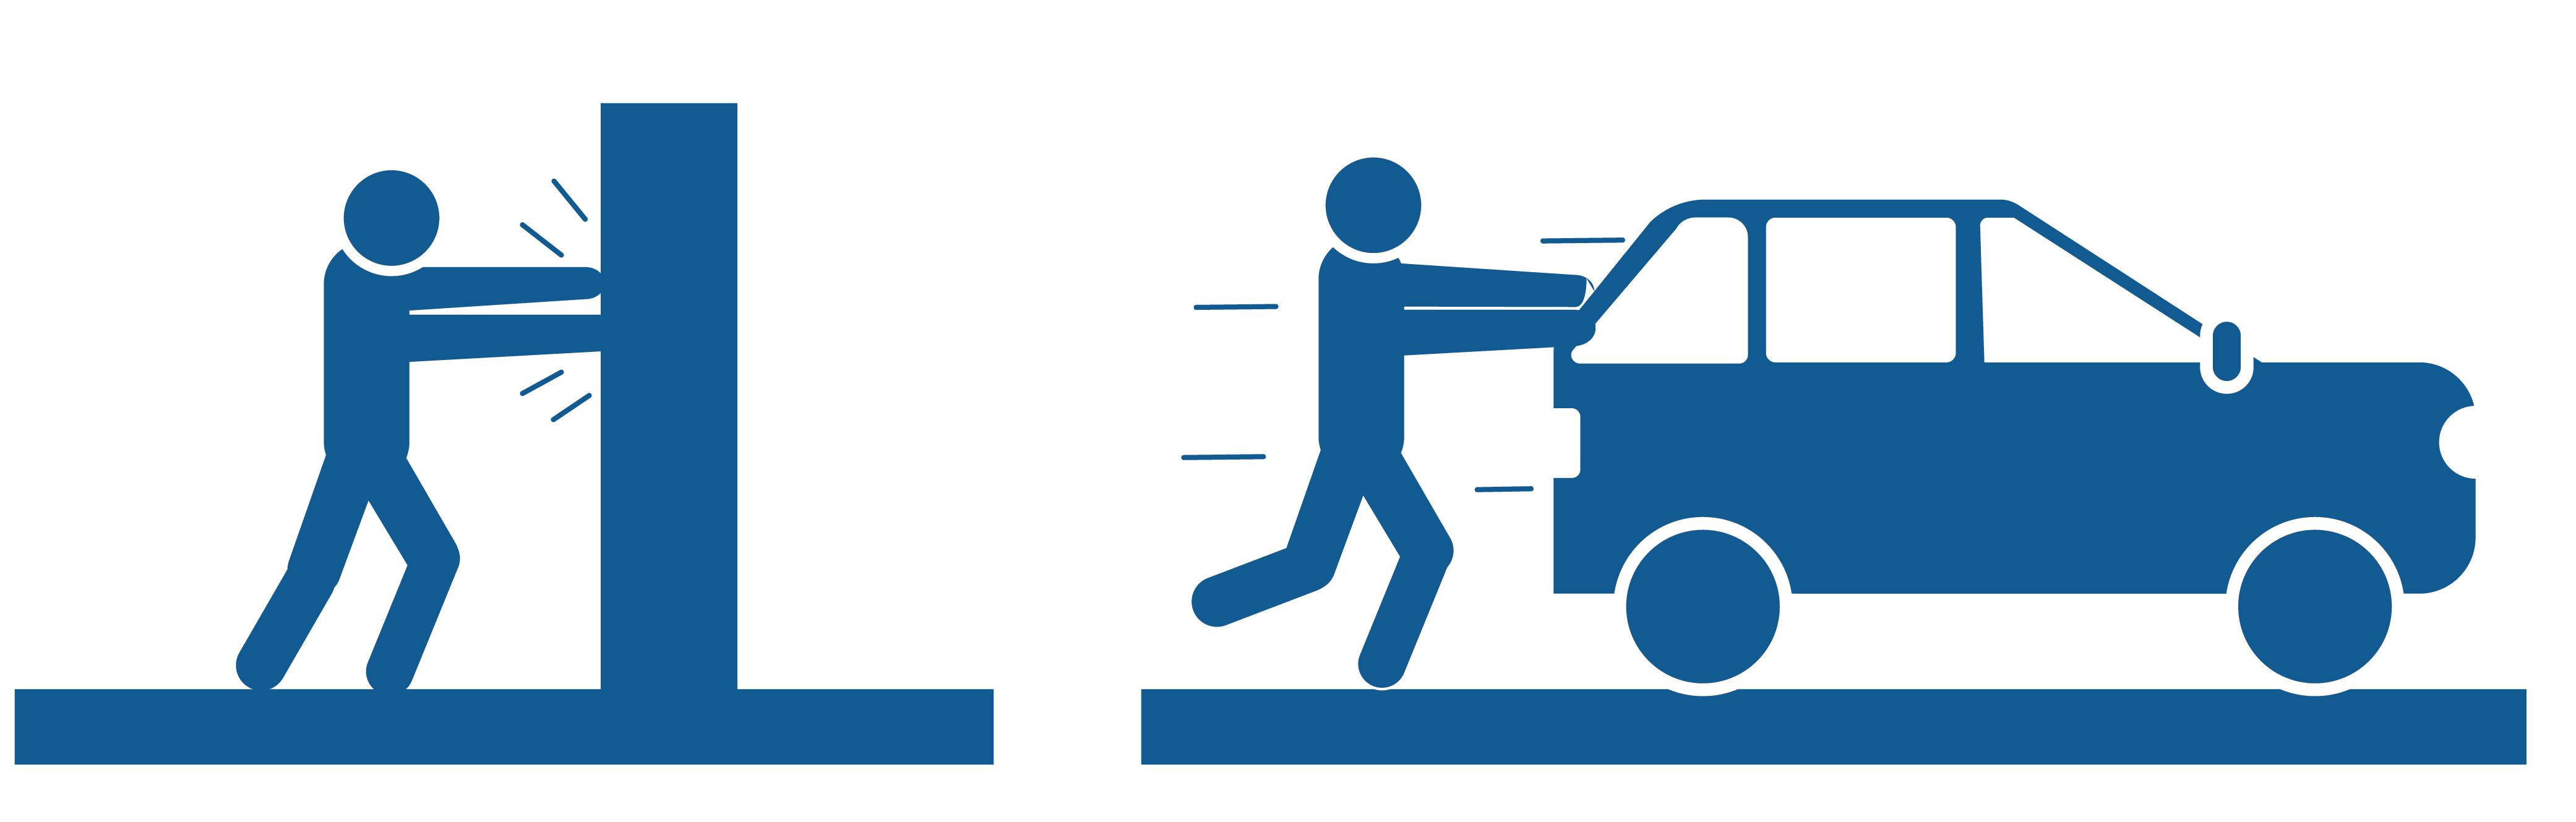
\includegraphics[width=0.6\textwidth]{workvsforce.png}
    \caption{Pushing on a wall does no work while pushing a car does work! Why?}
    \label{fig:workvsforce}
\end{figure}


For example, if you push a car with a force of 10 newtons for 12
meters, you have done 120 joules of work.\index{work}

\begin{mdframed}[style=important, frametitle={Formula for Work}]
If a force applied is \emph{constant}, the formulas for work is:
\[
W = F \cdot d
\]

where $W$ is the work in joules (N$\cdot$ m), $F$ is the \textit{force} in newtons, and $d$ is 
the distance in meters.

If the force is not in the same direction as the distance, we can use the cosine 
of the angle between the force and the distance:
\[
W = F \cdot d \cdot \cos(\theta)
\]

where $\theta$ is the angle between the force and the distance.
If the formula for work is \emph{not constant}, the formula becomes:
\[W = \int \textbf{F} \cdot \textbf{dr}\] where \textbf{dr} is an infinitesimal amount of displacement. An example of this kind of force is like a spring force, where the force varies with displacement.
\end{mdframed}

\begin{Exercise}[label=work1, title={Book done by a constant force}]
	\emph{This question is from an AP Physics C Review Book.}
	You slowly lift a 2 kg book at a \emph{constant velocity} through a distance of 3 m. How much work is done on the book?
\end{Exercise}
\begin{Answer}[ref=work1]
	In the case, the force you exert must balance the weight of the book, so $F=mg=2(9.8)= 19.6 N$. 
	Since this force is straight upward and the displacement is in the same direction, $W = F\cdot d = 19.6 \cdot 3 = 58.8 \, \text{J}$.
\end{Answer}

\index{work-energy theorem}The work-energy theorem (or work-energy principle) states that the net work done 
on an object is equal to the \textbf{change in its energy}. In other 
words, if you do work on an object, you are changing its energy. It follows from Newton's second law, which you met in the forces chapter. 

\[
W = \Delta E 
\]

Work is how energy is transferred from one thing to another. When you push the 
car, you also burn sugars (energy of the body) in your blood. That energy is then
transferred to the car after it has been pushed uphill.

Thus, we measure the energy something consumes or generates in units of work: 
joules, kilowatt-hours, horsepower-hours, foot-pounds, BTUs (British Thermal 
Unit), and calories.

Let us go over a few different forms that energy can take.

\section{Forms of Energy}\index{energy!Forms of}

In this section we are going to learn about several different types of energy:
\begin{itemize}
\item Heat
\item Electricity
\item Chemical Energy
\item Kinetic Energy
\item Gravitational Potential Energy
\end{itemize}

There are also other forms of energy such as \index{spring potential energy}spring potential energy, which we will cover in the oscillations chapter.
\subsection{Heat}\index{heat}

When you heat something, you are transferring energy to it. The BTU is a common 
unit for heat. One BTU is the amount of heat required to raise the temperature of 
one pound of water by one degree Fahrenheit. One BTU is about 1,055 joules. In fact, when 
you buy and sell natural gas as fuel, it is priced by the BTU.\index{heat} \index{BTU}

Friction is the most common way motion turns into heat. When friction does work, that energy shows up as heat in the surfaces that rub together.

\subsection{Electricity}\index{electricity}

Electricity is the movement of electrons. When you push electrons through a space 
that resists their passage (like a light bulb), energy is transferred from the 
power source (like a battery) into the source of the resistance.

Let us say your lightbulb consumes 60 \newterm{watts} of electricity, and you leave it on 
for 24 hours. You have used $60 \times 24 = 1{,}440$ watt-hours, or 1.44 \index{kilowatt-hour}kilowatt-hours, which is about 5,200,000 joules. Your electric bill, a car battery, and a phone battery are all rated this way. In an electric car, the battery's energy becomes kinetic energy, and friction eventually turns it into heat.\index{thermal energy}


\subsection{Chemical Energy}\index{chemical energy}

As mentioned earlier, some chemical reactions consume energy and some produce 
energy. This means energy can be stored in the structure of a molecule. When a 
plant uses photosynthesis to rearrange water and carbon dioxide into a sugar 
molecule, it converts the energy in the sunlight (solar energy) into chemical 
energy. Remember that photosynthesis is a process that consumes energy. 
Therefore, the sugar molecule has more chemical energy than the carbon dioxide 
and water molecules that were used in its creation.

Recall the balanced chemical equation for photosynthesis is:
\[
6 \text{CO}_2 + 6 \text{H}_2\text{O} + \text{energy} \rightarrow \text{C}_6\text{H}_{12}\text{O}_6 + 6 \text{O}_2
\]

% KA: https://www.khanacademy.org/science/ap-biology/cellular-energetics/photosynthesis/a/intro-to-photosynthesis -- added to digital resources

In our diet, we measure this energy in \textit{kilocalories}. A calorie is the 
energy necessary to raise one gram of water one degree Celsius, and is about 
4.19 joules. This is a very small unit. An apple has about 100,000 calories (100 
kilocalories), so people working with food started measuring everything in kilocalories.\index{calories}



Here is where things get tricky: People who work with food got tired of saying 
``kilocalories'', so they just started using ``Calorie'' to mean 1,000 calories. 
This has created a great deal of confusion over the years. So if the C is capitalized,
 ``Calorie'' probably means kilocalorie.

\subsection{Kinetic Energy}\index{kinetic energy}
A mass in motion has energy. For example, if you are in a moving car and you slam
on the brakes, the energy from the motion of the car is converted into heat in
the brake pads and under the tires. This stored energy of motion is known as
\emph{kinetic energy}.

But how much energy does a moving object actually have?

\begin{mdframed}[style=important, frametitle={Formula for Kinetic Energy}]
\[
KE = \frac{1}{2} m v^2
\]
where $KE$ is the kinetic energy in joules, $m$ is the mass in kilograms, and
$v$ is the speed in meters per second.
\end{mdframed}

This equation tells us two important things:

\begin{itemize}
  \item Kinetic energy increases \emph{linearly} with mass. A heavier object has
  more energy at the same speed.
  \item Kinetic energy increases \emph{quadratically} with velocity. This means
  that doubling the speed results in \emph{four times} the kinetic energy.
\end{itemize}

Where does $\frac{1}{2}mv^2$ come from? Push a mass $m$, starting from rest, with a constant force $F$ over a distance $d$. The work you do is $W = Fd = mad$. From kinematics, $v^2 = 2ad$, so $ad = \frac{1}{2}v^2$. Put those together: $W = \frac{1}{2}mv^2$. All the work you did became kinetic energy.

The $v^2$ explains why speed is so dangerous on the road. A car at 60 mph has four times the kinetic energy of the same car at 30 mph, so it needs four times the distance to stop with the same braking force, and it does four times the damage in a crash.

\begin{Exercise}[title={Kinetic and Thermal Energy}, label=energyBrakingCar]
  A $1,200 \text{ kg}$ car traveling at $22 \text{m/s}$ comes to a stop using its brakes.
  Assume all the initial kinetic energy is converted into thermal energy in the brakes and tires.

  \begin{enumerate}[label=(\alph*)]
    \item How much thermal energy, $Q$ is produced?
    \item If the brakes have a mass of $15 \text{ kg}$ and a specific heat of $c = 460 \text{ J/(kg}^\circ\text{C)}$, estimate their temperature increase.
  \end{enumerate}
  Use the fact that the temperature change is $\Delta T = \frac{Q}{m_{brake}c}$.
\end{Exercise}
\begin{Answer}[ref=energyBrakingCar]
  \begin{enumerate}[label=(\alph*)]
    \item Since all kinetic energy is transferred into thermal energy, we can say:
    \[Q = KE = \frac{1}{2}(1200)(22)^2 = 290,400 \text{ J}\]
    \item The rise in heat is given by $\Delta T = \dfrac{Q}{mc} = \frac{290,400}{15 \times 460} \approx 42^\circ \text{ C}$
  \end{enumerate}
\end{Answer}
\subsection{Gravitational Potential Energy}\index{potential energy!gravitational}


When you lift something heavy onto a shelf, you are giving it \textit{potential energy}. The amount of energy that you transferred to it is proportional to its 
weight and the height that you lifted it.

\begin{mdframed}[style=important, frametitle={Formula for Gravitational Potential Energy}]
The formula for gravitational potential energy is

\[
E = mgh
\]

where $E$ is the energy in joules, $m$ is the mass of the object you
lifted, $g$ is acceleration due to gravity, and $h$ is the height that you lifted it.

On earth, then, gravitational potential energy is given by

\[
E = (9.8)mh
\]

since objects in free-fall near Earth's surface accelerate at $9.8 m/s^2$.

\end{mdframed}


There are various kinds of potential energy. For example, when you draw a bow in 
order to fire an arrow, you have given that bow potential energy. When you release it, the potential energy is transferred to the arrow, which expresses it as kinetic energy. When you compress a spring, the energy put into the spring is proportional to the spring constant and distance it is compressed, $\frac{1}{2} kx^2$. We will dive deeper into this in the springs and oscillations chapter.


\section{Conservation of Energy}

The first law of thermodynamics says ``Energy is neither created nor destroyed.''
\index{energy!conservation of}

Energy can change forms. Your cells consume chemical energy to give gravitational potential energy to a car you push up a hill. A falling object converts potential energy into kinetic energy, causing it to speed up. However, the total amount of energy in a closed system stays constant. 

Kinetic plus potential energy is called \index{mechanical energy}mechanical energy. If nothing outside the system does work on it and nothing is lost to friction, the mechanical energy stays constant. In general, outside work changes the system's kinetic energy $K$, potential energy $U$, and thermal energy $E_\text{th}$:
\[
W_\text{net,ext}=\Delta E_\text{sys}=\Delta K+\Delta U+\Delta E_\text{th}
\]
Energy problems are bookkeeping problems. Pick your system, add up the energy at the start, add up the energy at the end, and account for every joule that came in or went out.

\begin{Exercise}[title={The Energy of Falling}, label=energy_falling]

A 5 kg cannonball falls off the top of a 3 meter ladder. As it falls, its 
gravitational potential energy is converted into kinetic energy. How fast is 
the cannonball traveling just before it hits the floor?

\end{Exercise}
\begin{Answer}[ref=energy_falling]

  At the top of the ladder, the cannonball has $(9.8)(5)(3) = 147 \text{ J}$ of potential energy.

  At the bottom, the kinetic energy $\frac{1}{2}(5)v^2$ must be equal
  to 147 joules. So $v^2 = \frac{294}{5}$.  This means it is going about
  $7.7 \text{ m/s}$.

  (You may be wondering about air resistance. Yes, a tiny amount of energy is 
  lost to air resistance, but for a dense object moving at these relatively slow 
  speeds, this energy is negligible.)

\end{Answer}

\begin{Exercise}[title=Frictional Losses, label =slidingblockfriction]
  A $4.0 \text{ kg}$ block is released from rest at the top of a rough incline of height $2.5 \text{ m}$.
  By the time it reaches the bottom, its speed is $4.2 \text{ m/s}$. 

  Determine the total mechanical energy lost to thermal energy.

  You may use $10 \text{ m/s}^2$ for g
\end{Exercise}
\begin{Answer}[ref=slidingblockfriction]
The initial total gravitational potential energy is $mgh = 4(10)(2.5) = 100 \text{ J}$. The final kinetic energy is $\frac{1}{2} mv^2 = \frac{1}{2}(4)(4.2)^2 = 35.28$. So, the rest of the energy must be lost due to friction: $100 - 35.28 = 64.72 \text{ J}$. 
\end{Answer}

\begin{Exercise}[title=Blast Off!, label=rocketsled]
  A rocket sled of mass $150 \text{ kg}$ uses a small fuel-powered booster that releases $1.2\times 10^5\,\text{J}$ of chemical energy. During the burn, $65\%$ of the energy is converted into useful kinetic energy for the sled, the rest is lost as heat or sound. Assume the sled travels on frictionless, smooth surface.

  Calculate the final speed of the rocket sled.
\end{Exercise}
\begin{Answer}[ref=rocketsled]
The total useful energy can be calculated as $0.65(1.2\times 10^5) = 7.8\times 10^4\,\text{J}$. Then, we can set the final KE $\frac{1}{2}mv^2 = 7.8\times 10^4$ and solve for $v$
\begin{align*}
  \frac{1}{2}(150)v^2 &= 7.8\times 10^4\\
  (150)v^2 &= 15.6 \times 10^4 \\ 
  v^2 &=1,040 \\ 
  v&\approx32.249 \text{ m/s}
\end{align*}
\end{Answer}

\subsection{Friction, Heat, and Energy "Loss"}
Imagine rolling a ball across a flat surface: you have given the ball some 
kinetic energy in its motion. If the kinetic energy were conserved, the ball 
would keep rolling at the same speed forever, as long as it was on a flat 
surface. Experience tells us this is not what happens: the ball will eventually 
come to a stop. Why does this not violate the conservation of energy?

Friction\index{friction} is the force that opposes motion: whenever you slide two objects past 
each other, friction transforms kinetic energy into heat. Rub the palms of your 
hands together. You should feel warmth, a product of the friction between your 
hands. As the ball in the example above rolls, it also experiences friction 
between itself and the ground. The friction slowly transforms the kinetic energy 
of the ball into heat, causing the ball to lose kinetic energy. When all of the 
ball's kinetic energy is transformed to heat, the ball comes to a rest. So, the 
kinetic energy of the ball was not destroyed and did not disappear: it became heat. 

In fact, nearly all energy in the universe will eventually be transformed to heat,
resulting in the inevitable ``heat death''\index{heat death of the universe} of the universe. (The Entropy and
the Second Law of Thermodynamics chapter explains why.) Here is a short video about heat, entropy, and the
heat death of the universe: \url{https://www.youtube.com/watch?v=gOWt_Hq3yrE/}. 

\subsection{Energy Conservation in Falling Objects}
Recall that an object above the ground has gravitational potential energy
$E_{p} = mgh$, where $m$ is the mass in kg, $g$ is the acceleration due to gravity 
($9.8 m/s^2$ on Earth), and $h$ is the height above the ground in meters.

\textbf{Example}: What is the gravitational potential energy of a 5.0 kilogram 
bowling ball in the hand of a bowler (approximately 1.2 meters high)?

\textbf{Solution}: The mass is 5.0 kg, the height is 1.2 m, and we assume the 
bowler is on Earth, so g is 9.8 $m/s^2$:

$$E_{p} = \left( 5.0 kg \right) \left( 9.8 m/s^2 \right) \left( 1.2 m \right) = 59 J$$

If the bowler were to drop that ball, it would lose potential energy and gain 
kinetic energy, $E_{k} = \frac{1}{2}mv^2$. If there is no air resistance, then as an object falls 
all of its potential energy is converted to kinetic energy. (If you'd like to 
explore what happens when friction is accounted for, you can play with this PhET 
simulation: \url{https://phet.colorado.edu/en/simulations/energy-skate-park}.)

\textbf{Example}: If the bowling ball were dropped, what would its speed be right 
before it hits the ground? (Neglect air resistance.)

\textbf{Solution}: Ignoring air resistance, according to the Law of Conservation 
of Energy, the kinetic energy of the ball right before it hits the ground must be 
equal to the gravitational potential energy of the ball right before its release. 
Therefore:

$$mgh = \frac{1}{2}mv^2$$

We can eliminate an $m$ from both sides and rearrange to solve for $v$:

$$v = \sqrt{2gh} = \sqrt{2 \left( 9.8 m/s^2 \right) \left(1.2 m \right)} = 
\sqrt{23.52 \frac{m^2}{s^2}} = 4.8 \frac{m}{s}$$

The ball will have a speed of 4.8 m/s just before it hits the ground. 

\begin{Exercise}[title = {Kinetic and Potential Energy}, label = ke_pe]
\begin{enumerate}
\item How fast should you toss a ball straight up if you want it to reach your 
friend on the second floor (3.7 meters above you)?
\item Your little brother is teasing you from a treehouse 5.0 meters off the 
ground. If your slingshot can shoot a pebble at 15 m/s, can you hit your little 
brother?
\item A 63-kg roller-blader rolls down a hill. If the hill is 8.0 meters high and 
they reach the bottom of the hill with a speed of 11.2 m/s, how much energy was 
converted to heat through friction?
\end{enumerate}
\vspace{25mm}
\end{Exercise}

\begin{Answer}[ref = ke_pe]
\begin{enumerate}
\item $v = \sqrt{2gh} = \sqrt{2 \left( 9.8 m/s^2 \right) \left( 3.7 m \right)} = 
8.5 m/s$
\item $h = \frac{v^2}{2g} = \frac{\left( 15 \frac{m}{s} \right)^2}{2 \left( 9.8 
\frac{m}{s^2} \right)} = 11.5 m$. You can hit your little brother, since you could 
shoot the pebble as high as 11.5 m and he is only 5.0 m above you.
\item We know that $E_{p, initial} = E_{k, final} + E_{lost to friction}$. 
Therefore, $E_{lost\_to\_friction} = E_{p, initial} - E_{k, final} = mgh - \frac{1}{2}
mv^2 = \left(63 kg \right) \left( 9.8 \frac{m}{s^2} \right) \left( 8 m \right) -
\frac{1}{2} \left( 63 kg \right) \left( 11.2 \frac{m}{s} \right)^2 = 4939.2 J - 
3951.4 J = 988 J$. 
\end{enumerate}
\end{Answer}

\section{Types of Systems}
We classify systems based on the flow of matter and energy. A \textit{system} is 
a set of interconnected elements. Your body is a system, as is a television or a 
boiling pot of water. Scientists define systems by separating the parts of the 
system from the rest of the universe, usually called "the surroundings". You can 
represent this separation with a dashed line. Here is a diagram defining a pot of
boiling water as a system:

\begin{center}
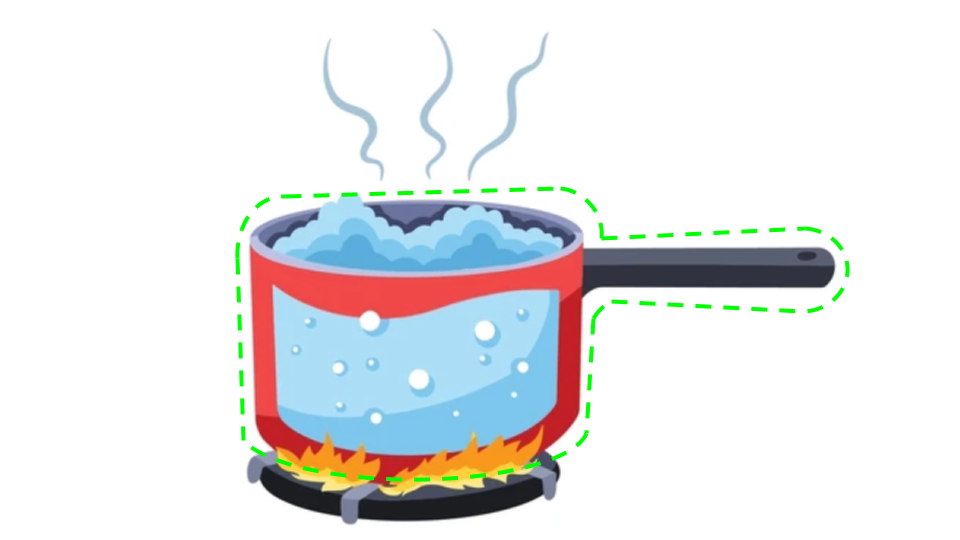
\includegraphics[width=4in]{pot_open_system.png}
\end{center}

Everything inside the dashed line is the system: the pot and the water boiling in
it. Everything outside the dashed line is the surroundings: the stove, the air 
around the pot, etc. Defining a system is \textit{arbitrary}: there is not one hard 
and fast definition of a system. Think of your school: you could look at the 
system of a classroom, the system of a hallway and all the classes connected to 
it, or the entire school building. How you define a system depends on what you are 
studying. 

\subsection{Open Systems}
An \textit{open system} allows for matter and energy to cross the imaginary 
boundary between the system and its surroundings. The uncovered pot of boiling 
water is an example of an open system. Energy enters the system as heat from the
stove, and leaves the system as heat in the steam rising from the pot. Notice 
that steam rising: see how it crosses the imaginary boundary? The steam is matter 
\textit{leaving the system}. Since matter and energy can cross the boundary 
between the system and its surroundings, the uncovered boiling pot is an open 
system. \index{open system}

\begin{center}
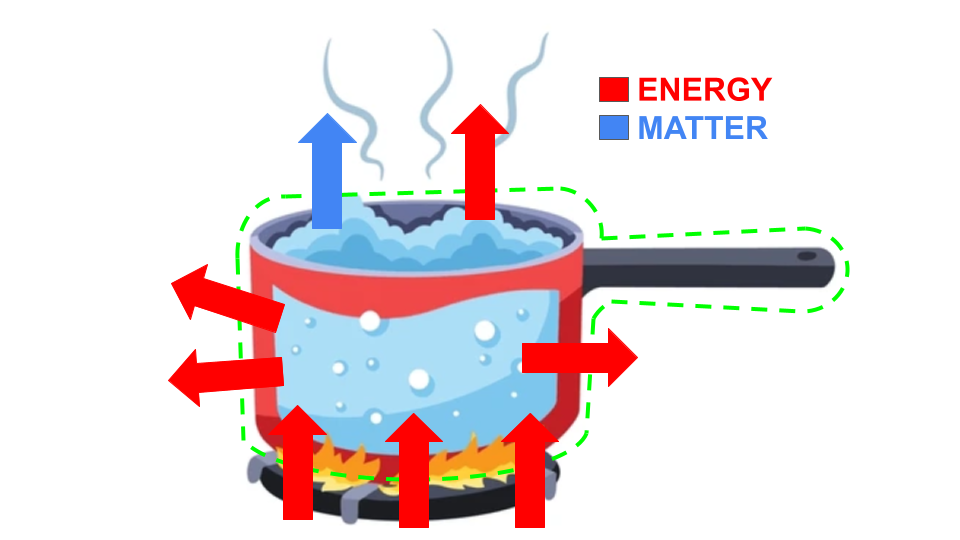
\includegraphics[width=4in]{pot_open_arrows.png}
\end{center}

The system also loses energy through the sides of the pot: if you touched the 
pot, it would feel hot, which means heat energy can also leave the system through
the sides of the pot. This is due to the collision between air particles (the 
surroundings) and the outside of the pot (the system). With every collision, a 
little heat is transferred from the pot to the air. This is why your hot drink 
gets cold if you leave it out, even if you do not add any ice. 

\subsection{Closed Systems}
A \textit{closed system} allows for the transfer of energy but not the transfer 
of matter. If we put a lid on this pot, it would become a closed system. 
\index{closed system}

\begin{center}
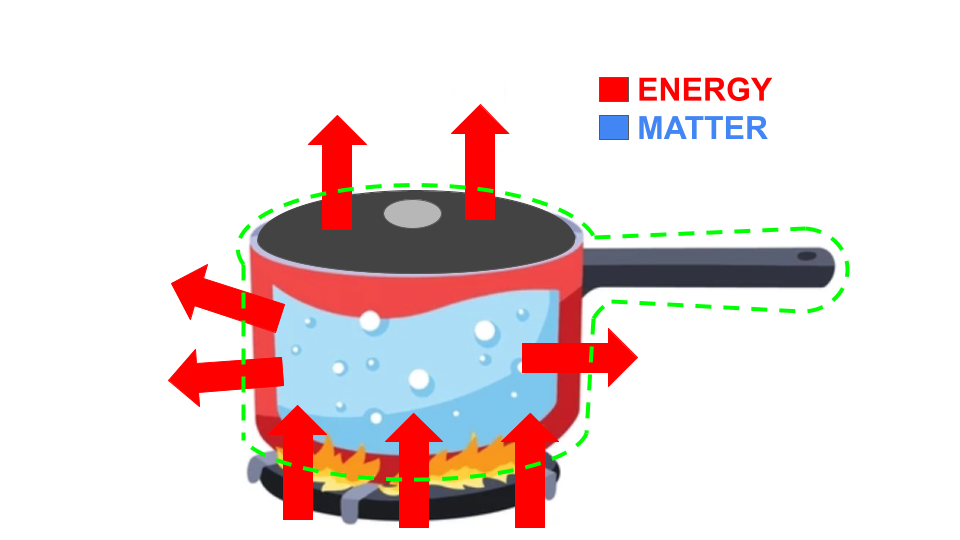
\includegraphics[width=4in]{pot_closed_system.png}
\end{center}

Notice that the difference between an open and closed system is the flow of 
\textit{matter}: open systems allow for the movement of matter, while closed 
systems do not. However, energy can still enter and leave closed systems. 
Sealed containers that are not insulated are good examples of closed systems - 
a car with the windows up and doors closed. 

\subsection{Isolated Systems}
An \textit{isolated system}\index{isolated system} does not allow for the flow of matter \textit{or} 
energy in or out of the system. There is no such thing as a truly isolated system: in reality, a small amount of energy can be transferred even through the best 
thermal insulators. However, for well-insulated systems, it can be a good 
approximation to model that system as isolated. A simple example would be a 
sealed, well-insulated coffee thermos. The transfer of heat energy between the 
coffee in the thermos and the thermos' surroundings is so slow that we can ignore
that small amount of transfer and approximate the thermos as an isolated system. 

\subsection{Classifying Systems}
To quickly categorize a system as open, closed, or isolated, ask yourself two questions:
\begin{enumerate}
\item Can matter enter or leave the system?
\item Can energy enter or leave the system?
\end{enumerate}

If your answer to the first question is yes, you know automatically the system 
is open. If no, move to the second question. If energy can enter or leave, the 
system is closed. If not, the system is isolated. Sometimes, textbooks and exams 
will describe a system as "well-insulated". This is directing you to assume any 
transfer of energy between the system and surroundings is negligible, and that 
you should treat the system as an isolated system. 

\begin{Exercise}[title = {Open, Closed, and Isolated Systems}, label = systems]
Classify each system as open, closed, or isolated. Justify your answer. 
\begin{enumerate}
\item The human body
\item Earth
\item Your cell phone
\item A well-insulated cooler with the lid sealed
\item A well-insulated cooler with the lid open
\item A bottle of soda before it is opened to be drunk
\end{enumerate}
\end{Exercise}

\begin{Answer}[ref = systems]
\begin{enumerate}
\item The human body is an open system because matter can enter (food, water, 
oxygen) and leave (waste, carbon dioxide, sweat) your body.
\item The Earth is an open system because matter can enter (asteroids falling, 
spaceships returning) and leave (space vehicles and astronauts). On the other 
hand, the Earth can be well-approximated as a closed system. Before the 20th 
Century, humans had no way to deliberately expel matter from the Earth, and the 
mass of asteroids that are pulled in by the Earth's gravity is negligible 
compared to the Earth. Therefore, in the right circumstances, it would be 
appropriate to model the Earth as a closed system. (It is closed because 
energy in the form of sunlight is constantly entering the system.)
\item A cell phone is a closed system - you do not put any matter in or take it 
out of your phone, but it constantly uses battery and then is recharged, showing
that energy enters and leaves your phone. 
\item Since the cooler is described as well-insulated and the lid is closed, it 
can be approximated as an isolated system. Scientific equipment, like bomb 
calorimeters, rely on this approximation. 
\item With the lid open, matter can enter and leave and therefore the cooler is 
an open system (yes, even though it is well-insulated). 
\item A sealed bottle of soda is a closed system - the soda and carbon dioxide 
cannot escape, but energy in the form of heat can be transferred in and out of 
the system (the contents of the bottle will lose heat if you put it in the 
fridge and gain heat if you leave it in the sun).
\end{enumerate}
\end{Answer}

\section{Mass-Energy Equivalence}
You have probably seen the equation
$$E = mc^2$$

$E$ is energy, $m$ is mass, and $c$ is the speed of light in a vacuum (about $3 
\times 10^8 \frac{m}{s}$). In the Atoms and Matter chapter, mass was conserved; in this chapter, energy
is conserved. This equation shows that the two are connected: matter can be
converted to energy, and vice versa.\index{mass-energy equivalence} This is the source of the light energy emitted by the sun. 

The Sun is mostly hydrogen. At the very center, it is so hot and dense that the 
nuclei of hydrogen atoms are fused together to form helium atoms, a process 
called the \textit{proton-proton chain reaction}. The actual reaction involves several 
steps and is more complicated, but the overall process can be summarized as:

$$4\text{H} \to \text{He}$$

If every hydrogen atom has a mass of approximately $1.6735575 \times 10^{-27}$ kg 
and every helium atom has a mass of approximately $6.6464731 \times 10^{-27}$ kg, 
how much energy is released when one atom of helium is created? First, notice 
that one helium has less mass than 4 hydrogen atoms:

$$4 \times \left( 1.6735575 \times 10^{-27} \right) - 6.6464731 \times 10^{-27} = 
4.77569 \times 10^{-29}$$

Now, we can use $E = mc^2$ to find out how much energy is equivalent to $4.77569 
\times 10^{-29}$ kg:

$$E = \left( 4.77569 \times 10^{-29} \text{kg} \right) \left( 2.99792458 \times 
10^8 \frac{\text{m}}{\text{s}} \right)^2$$
$$E \approx 4.292 \times 10^{-12} \text{joules}$$

That is a tiny number, so let us scale up. Suppose you fused 1 kilogram of hydrogen (as a gas, enough to fill a small bedroom). The lost mass is $\frac{4.77569 \times 10^{-29}}{4 \times 1.6735575 \times 10^{-27}} \approx 0.71\%$ of the hydrogen's mass, so about 0.00713 kg disappears, roughly the mass of three pennies.

$$E = \left( 0.00713 \text{ kg} \right) \left( 2.99792458 \times 10^8 \frac{
\text{m}}{\text{s}} \right)^2 \approx 6.4 \times 10^{14} \text{ joules}$$

That is about 180,000,000 kWh (kilowatt-hours). An average US home uses about 30 kWh per day, so one kilogram of hydrogen could power a home for \textit{over 16,000 years}! That is why scientists keep working on nuclear fusion power. The nuclear power plants currently running around the world 
today rely on \textit{nuclear fission}\index{nuclear fission}: the splitting apart of atoms, the opposite
process of \textit{nuclear fusion}.\index{nuclear fusion} Fission releases several times less energy 
per kilogram of fuel than fusion, and thus stable, affordable 
nuclear fusion power plants remain a ``holy grail'' of scientific research. The Nuclear Physics and
Radioactivity chapter explains fission and fusion in detail.

The next chapter, Work, Kinetic Energy, and Power, connects work directly to an object's speed, and asks
how efficiently and how quickly energy gets a job done.
